\PassOptionsToPackage{table}{xcolor}

\documentclass[aspectratio=169]{beamer}

\usetheme{auriga}
\usecolortheme{auriga}
\setbeamersize{text margin left=2em,text margin right=2em}

\usepackage{fontspec}
\usepackage{xcolor}
\usepackage{enumitem}
\usepackage{makecell}
\usepackage{tabularx}
\usepackage[outputdir=build, newfloat]{minted}
\usepackage{unicode-math}
\usepackage{animate}
\usepackage{amsmath}
\usepackage{ulem}
\usepackage[russian]{babel}

\setminted{
  fontsize=\scriptsize,
  baselinestretch=1.5
}

% for vertical centering text in X column
\renewcommand\tabularxcolumn[1]{m{#1}}
\newcolumntype{C}{>{\centering\arraybackslash}X}

\setmainfont{PT Astra Serif}

\makeatletter
\AddEnumerateCounter{\asbuk}{\russian@alph}{щ}
\makeatother

\title{
  \huge{
    Медиазапросы в CSS
  }
}
\author{Швалов Даниил К33211}
\institute{Университет ИТМО}
\date{2023}

\begin{document}

% change itemize default label
\def\labelitemi{---}

\frame{\titlepage}

\begin{frame}
  \frametitle{Зачем нужны медиазапросы}

  \begin{columns}[onlytextwidth,c]
    \column{0.6\textwidth}

    Представим, что мы разрабатываем веб-приложение, целевая аудитория которого
    использует различные виды устройств, например, персональные компьютеры и
    смартфоны.

    \vspace*{1em}

    При этом мы не обладаем достаточными ресурсами, чтобы разработать
    различные клиенты для всех видов устройств. Поэтому нам нужно каким-то
    образом сделать так, чтобы один и тот же веб-сайт корректно работал на всех
    устройствах.

    \vspace*{1em}

    Для решения этой проблемы используются \textbf{медиазапросы}.

    \column{0.4\textwidth}

    
\includegraphics[width=\textwidth]{images/responsive-design.png}
  \end{columns}
\end{frame}

\begin{frame}[fragile]
  \frametitle{Синтаксис медиазапросов}

  Медиазапрос начинается с ключевого слова \textbf{@media} после которого
  указывается одно или несколько условий. В качестве условия можно указывать тип
  устройства или требования к определённой характеристике, которые записываются
  в круглых скобках.

  \vspace*{1em}

  \begin{minted}{css}
  @media (min-width: 992px) and (max-width: 1200px) {
    /* стили будут применяться, когда условие истинно */
  }
  \end{minted}
\end{frame}

\begin{frame}[fragile]
  \frametitle{Логические операторы}

  В медиазапросах можно использовать логические операторы для комбинирования
  различных условий.

  \vspace*{1em}

  Виды логических операторов:
  \begin{itemize}
    \item \textbf{and} возвращает \textbf{true}, если каждая из характеристик
    является истинным, иначе \textbf{false}.
    \item \textbf{not} возвращает \textbf{true}, если характеристика является
    ложной, иначе \textbf{false}.
    \item \textbf{only} предназначено для того, чтобы браузеры, которые не
    поддерживают CSS3 медиазапросы, их игнорировали. В настоящее время это уже
    не актуально, поэтому использовать only не нужно.
    \item \textbf{,} или \textbf{or} возвращают \textbf{true}, если хотя бы
    один из характеристик является истинной, иначе \textbf{false}.
  \end{itemize}
\end{frame}

\begin{frame}[fragile]
  \frametitle{Типы устройств}

  В медиазапросах можно указывать определённые типы устройств:
  \begin{itemize}
    \item \textbf{all} --- для всех;
    \item \textbf{screen} --- для устройств с экранами;
    \item \textbf{print} --- для принтеров и в режиме предварительного просмотра
    страницы перед печатью;
    \item \textbf{speech} --- для программ чтения с экрана.
  \end{itemize}

  \vspace*{1em}

  Пример медиазапроса:
  \begin{minted}{css}
  @media screen and (max-width: 1200px) { /* ... */ }
  \end{minted}
\end{frame}

\begin{frame}[fragile]
  \frametitle{Характеристики}

  При составлении условия кроме типов устройств и логических операторов можно
  ещё задавать требования к определённым характеристикам.  

  \vspace*{1em}

  Самыми используемыми характеристиками являются \textbf{width} и
  \textbf{height}, а также их вариации \textbf{min-width}, \textbf{max-width},
  \textbf{min-height}, \textbf{max-height}. Примеры использования:

  \begin{minted}{css}
  @media (width: 320px) { /* ... */ }

  @media (min-width: 800px) and (max-width: 1200px) { /* ... */ }

  @media (min-height: 600px) { /* ... */ }
  \end{minted}
\end{frame}

\begin{frame}[fragile]
  \frametitle{Характеристика orientation}

  С помощью характеристики \textbf{orientation} можно установить те или иные
  стили в зависимости от того, в каком режиме (альбомном или портретном)
  отображается сайт. Примеры использования:

  \begin{minted}{css}
  @media (orientation: landscape) { /* ... */ }

  @media (orientation: portrait) { /* ... */ }
  \end{minted}
\end{frame}

\begin{frame}[fragile]
  \frametitle{Характеристика aspect-ratio}

  Характеристики \textbf{aspect-ratio}, \textbf{min-aspect-ratio} и
  \textbf{max-aspect-ratio} позволяют задавать стили в зависимости от
  соотношения сторон. Примеры использования:

  \begin{minted}{css}
  @media (min-aspect-ratio: 9/16) { /* ... */ }

  @media (max-aspect-ratio: 16/9) { /* ... */ }

  @media (aspect-ratio: 1/1) { /* ... */}
  \end{minted}
\end{frame}

\begin{frame}[fragile]
  \frametitle{Характеристика hover}

  Характеристика \textbf{hover} позволяет определить, поддерживает ли клиент
  наведение курсора на элементы. Она принимает два значения: \textbf{hover}
  (поддерживает) и \textbf{none} (не поддерживает). Примеры использования:

  \begin{minted}{css}
  @media (hover: hover) { /* ... */ }

  @media (hover: none) { /* ... */ }
  \end{minted}
\end{frame}

\begin{frame}
  \frametitle{Пример HTML-страницы}

  \inputminted{html}{examples/simple/index.html}

\end{frame}

\begin{frame}
  \frametitle{Пример CSS с медиазапросом}

  \inputminted{css}{examples/simple/styles.css}
\end{frame}

\begin{frame}
  \frametitle{Пример работы медиазапроса}

  \centering
  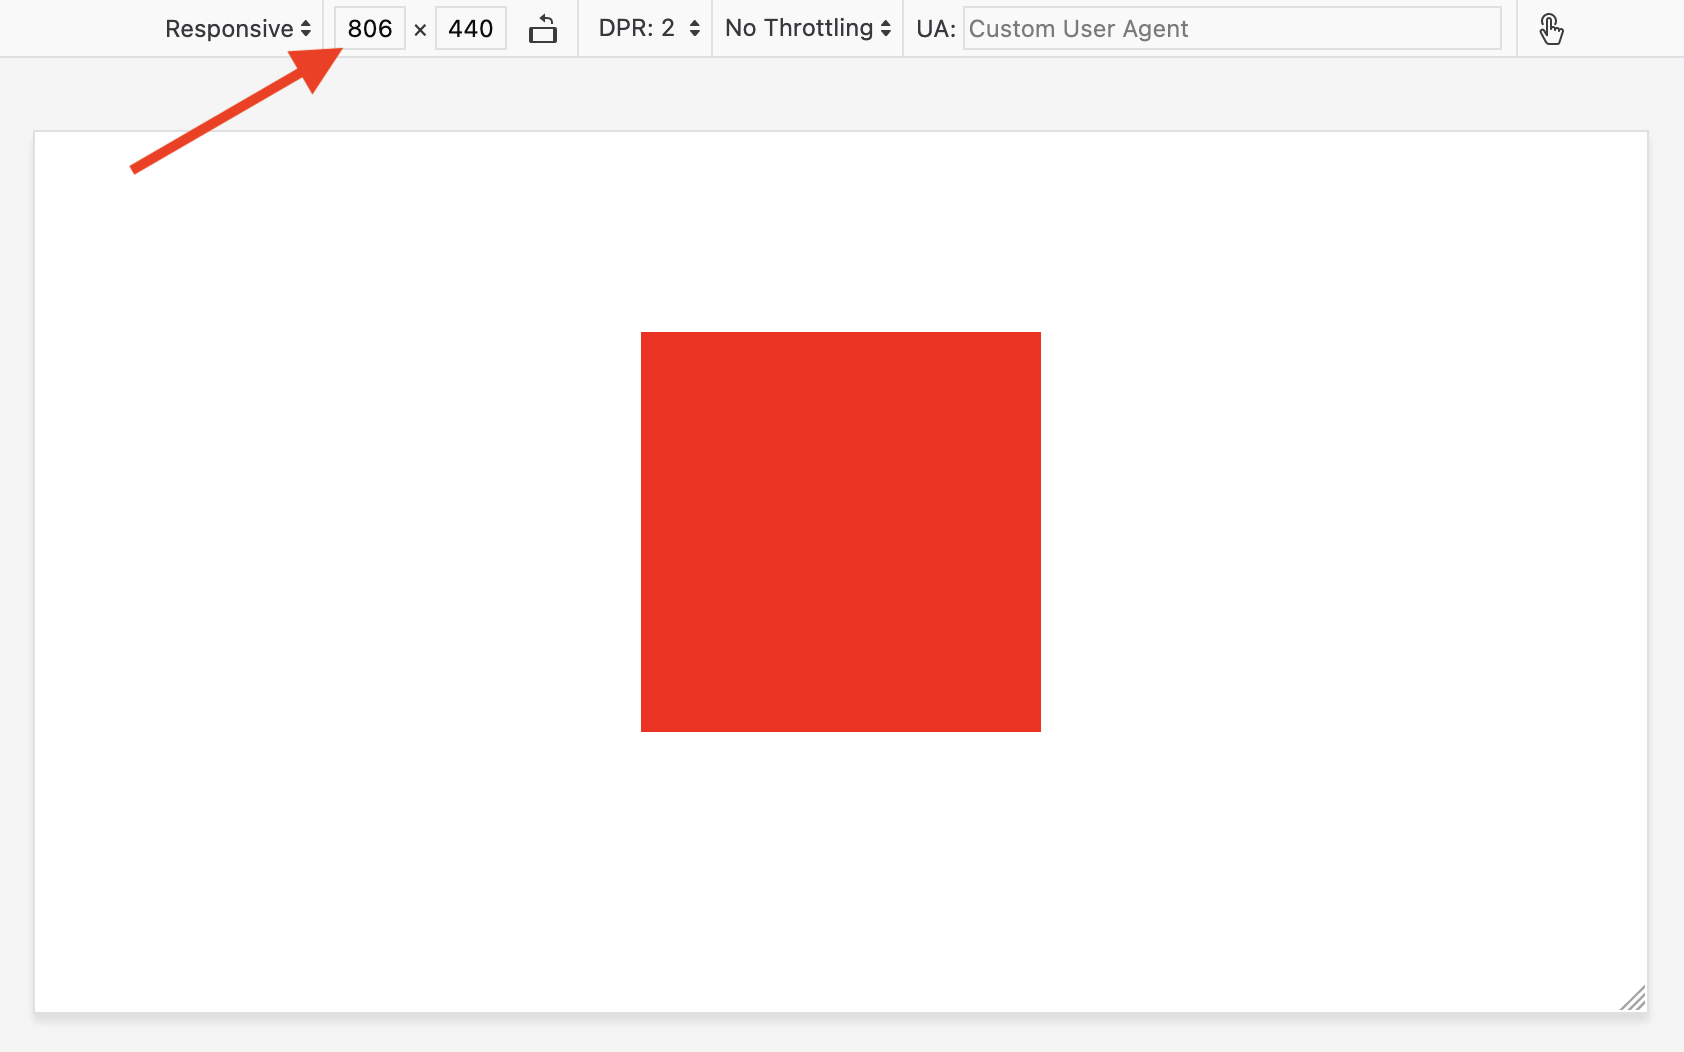
\includegraphics[width=0.75\textwidth]{images/box-example-1.png}
\end{frame}

\begin{frame}
  \frametitle{Пример работы медиазапроса}

  \centering
  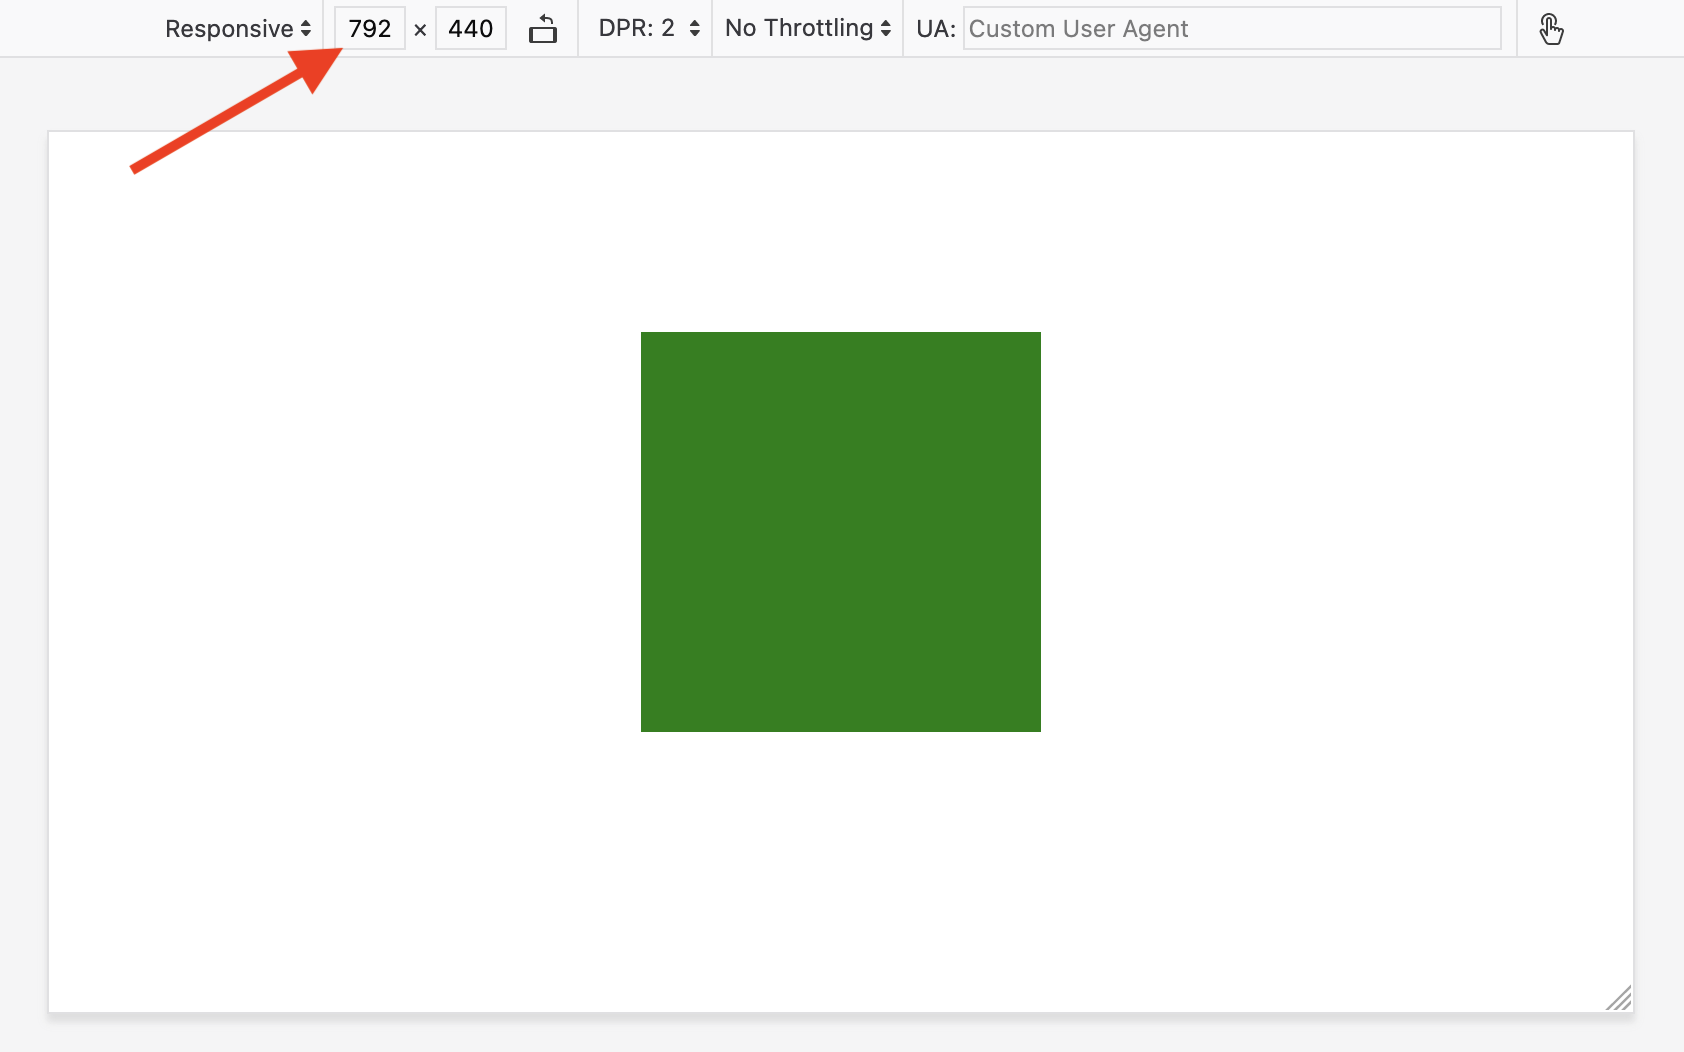
\includegraphics[width=0.75\textwidth]{images/box-example-2.png}
\end{frame}

\begin{frame}
  \begin{center}
    {\huge \textbf{Время для теста}}

    \vspace*{1em}

    \sout{$\text{Достаем двойные листочки}$}

    \vspace*{1em}

    
\includegraphics[width=0.35\textwidth]{images/form-qr.png}
  \end{center}
\end{frame}

% \begin{frame}
%   \frametitle{Вопрос №1}

%   Для чего используются медиазапросы в CSS?

%   \vspace*{2em}

%   \textbf{Варианты ответов}:
%   \begin{enumerate}[label=\asbuk*),ref=\asbuk*]
%     \item Для выполнения сетевых запросов по протоколу TCP/UDP, а также других
%     любых протоколов, которые поддерживаются браузером.
%     \item Для загрузки медиа-файлов (картинок, видео и т. п.) с удаленного
%     сервера.
%     \item Для управления стилями в зависимости от значений технических
%     параметров устройств (размер экрана и т. п.).
%     \item В качестве нового скриптового языка вместо JavaScript, который был
%     объявлен устаревшим.
%   \end{enumerate}
% \end{frame}

% \begin{frame}
%   \frametitle{Вопрос №2}

%   Какого типа устройств не существует в медиазапросах?

%   \vspace*{2em}

%   \textbf{Варианты ответов}:
%   \begin{enumerate}[label=\asbuk*),ref=\asbuk*]
%     \item print
%     \item screen
%     \item mobile
%     \item speech
%   \end{enumerate}
% \end{frame}

% \begin{frame}
%   \frametitle{Вопрос №3}

%   Какого логического оператора не существует в медиазапросах?

%   \vspace*{2em}

%   \textbf{Варианты ответов}:
%   \begin{enumerate}[label=\asbuk*),ref=\asbuk*]
%     \item and
%     \item only
%     \item ,
%     \item has
%   \end{enumerate}
% \end{frame}

% \begin{frame}
%   \frametitle{Вопрос №4}

%   Для чего используется характеристика \textbf{orientation}?

%   \vspace*{2em}

%   \textbf{Варианты ответов}:
%   \begin{enumerate}[label=\asbuk*),ref=\asbuk*]
%     \item Для проверки того, какой пол у пользователя (мужской, женский,
%     другой, не указан) указан в браузере.
%     \item Для проверки того, какая ориентация экрана пользователя (портретная
%     или альбомная ориентация).
%     \item Для проверки того, какое отношение сторон у экрана пользователя (16:9,
%     4:3 и т. п.).
%     \item Данной характеристики не существует в CSS.
%   \end{enumerate}
% \end{frame}

% \begin{frame}[fragile]
%   \frametitle{Вопрос №5}

%   Для чего используется данный медиазапрос?

%   \begin{minted}{css}
%   @media (hover: hover) { /* ... */ }
%   \end{minted}

%   \vspace*{1em}

%   \textbf{Варианты ответов}:
%   \begin{enumerate}[label=\asbuk*),ref=\asbuk*]
%     \item Для проверки того, что клиент поддерживает наведение курсором.
%     \item Для проверки того, что на странице есть элемент с классом <<hover>>.
%     \item Для проверки того, что CSS-переменная <<hover>> имеет значение
%     <<hover>>.
%     \item Для проверки того, что у клиента есть доступ к серверу с именем
%     <<hover>>.
%   \end{enumerate}
% \end{frame}

\end{document}
